\section{Goal of the project}
\label{sec:goalofproject}
%\minitoc
%\printinunitsof{cm}\prntlen{\textwidth}
%\printinunitsof{cm}\prntlen{\textheight}

The interaction of aerodynamics and structures is a key feature in aircraft design. Coupled aeroelastic analyses allow a better prediction of the aerodynamic forces and structural displacements that the aircraft experiences in real flight. High fidelity CFD analyses offer accurate results, but at the expense of high computational time. On the other hand, potential flow theory, and its computational implementation, the panel codes, offer reasonable approximations with low computational demands. The main goal of this project is to efficiently use low-fidelity analyses, combined to high-fidelity ones, to conduct aeroelastic optimizations, with an application to a Blended Wing Body (BWB) configuration.

\section{Project issues}
\label{sec:projectissues}
The development of a multifidelity method for aeroelastic analysis requires a coordinated implementation fo the high-fidelity and low-fidelity models. In order to achieve this, a management strategy must be implemented. Commonly used alternatives include: Trust Region Model Management (TRMM), Bayesian Regression, Cokringing \cite{peherstorfer2018survey}. Another important part of this step is to define the criteria that trigger the alternation between fidelities.

Once a management strategy has been chosen, the next step is to implement said model in the OpenMDAO platform. The resulting code has to be applicable to general cases in order to ensure its application a wide variety of problems and not just the particular aeroelastic case discussed in this work. Finally, the multifidelity method has to be applied to the aeroelastic optimization of a Blended Wing Body. The main issue at this point is the validation of the results because there are few well documented cases of BWB concepts that can be used as reference for the present work. 


\section{Main bibliography and state of the art}
\label{sec:unchapitre}
The starting point for the bibliography research is a Survey of Multifidelity Methods by Peherstorfer \cite{peherstorfer2018survey}, where a variety of alternatives are listed and classified. Surrogate modelling is a global optimization strategy. It uses co-kringing as a regression technique in order to link High-Fidelity sources with one or many Low-Fidelity functions. This
correlated model can be used to find optimal solutions more quickly \cite{Forrester2007}. On the other hand, simpler approaches such as a linear regression are found to offer a good balance between accuracy, cost and simplicity \cite{Zhang2019}. Other advantages include: ease to combine many low-fidelity sources and robustness for High-Fidelity samples with the presence of noise \cite{Zhang2019}. 

Newton methods and their variations have been explored as well. Jovanov and Breuker propose to solve the High-Fidelity problem by adding an aerodynamic correction load to the solution of the Low-Fidelity equation. The defect-correction method accelerates the convergence compared to the Quasi-Newton method \cite{Jovanov2015}. This last case does not consider the methods as black-boxes, but rather exploits the fact that the algorithms of both fidelity levels are known and can be modified at any stage to accommodate the necessary corrections between them. Scholz presents an Aggressive Space Mapping methodology, it solves for the low fidelity fluid–structure interaction solution and then feeds that information to a Quasi-Newton algorithm. The final results are obtained from a mapping function between both fidelity levels \cite{Scholcz2014}. 

When it comes to the application of mutifidelity models to aerospace design, there are several publications on the subject. A Bayesian-enhanced Low-Fidelity correction proved the ability to maintain high-fidelity accuracy while reducing
computational cost associated with the optimization of an airfoil shape \cite{fischer2018bayesian}. An aeroelastic optimization of a BWB was carried out by Bryson \cite{Bryson2019} using a new TRMM approach. Its main difference is that it adds hybrid additive-multiplicative corrections (or bridge functions) to the low-fidelity analysis \cite{Bryson2019a}. Another approach to the aeroelastic optimization of a BWB is presented by Marques \cite{Marques2019}. The flutter boundary problem is solved with a contour location approach (i.e. the zero contour of the aeroelastic damping coefficient). It also incorporates an active learning strategy, where the model evaluations are selected iteratively based on how much they are estimated to improve the predictions. 


\section{Milestones of the project}
\label{sec:milestones}
The milestones of the project are described below. A Gantt chart of the project is shown in fig. \ref{fig:gantt}.
\begin{itemize}
    \item Complete revision of the state of the art: 30/04/2019
    
    A thorough review of the pertinent bibliography is completed, as well as its written summary for the report.
    \item Definition of the management model between fidelities: 15/05/2019
    
    As a result of the research on the state of the art, a management algorithm is chosen and defined for the multifidelity method. The development of the code starts right after this definition.
    \item First working program for a test function: 15/09/2019.
    
    The multifidelity method is used to optimize a test function in order to ensure the functionality of the program. 
    \item Implementation of the method for a BWB case: 01/12/2019.
    
    The Blended Wing Body case is modelled and analyzed using the multifidelity aeroelastic optimization tool and the results are compared with documented sources.
    \item First draft of the complete report: 01/02/2020.
    
    An integration of the results, source code, methodology and conclusions is carried out. This first draft is then sent to the project supervisors for feedback.
    \item Report ready for final submission: 15/03/2020.
\end{itemize}
\begin{sidewaysfigure}[htpb]
\centering
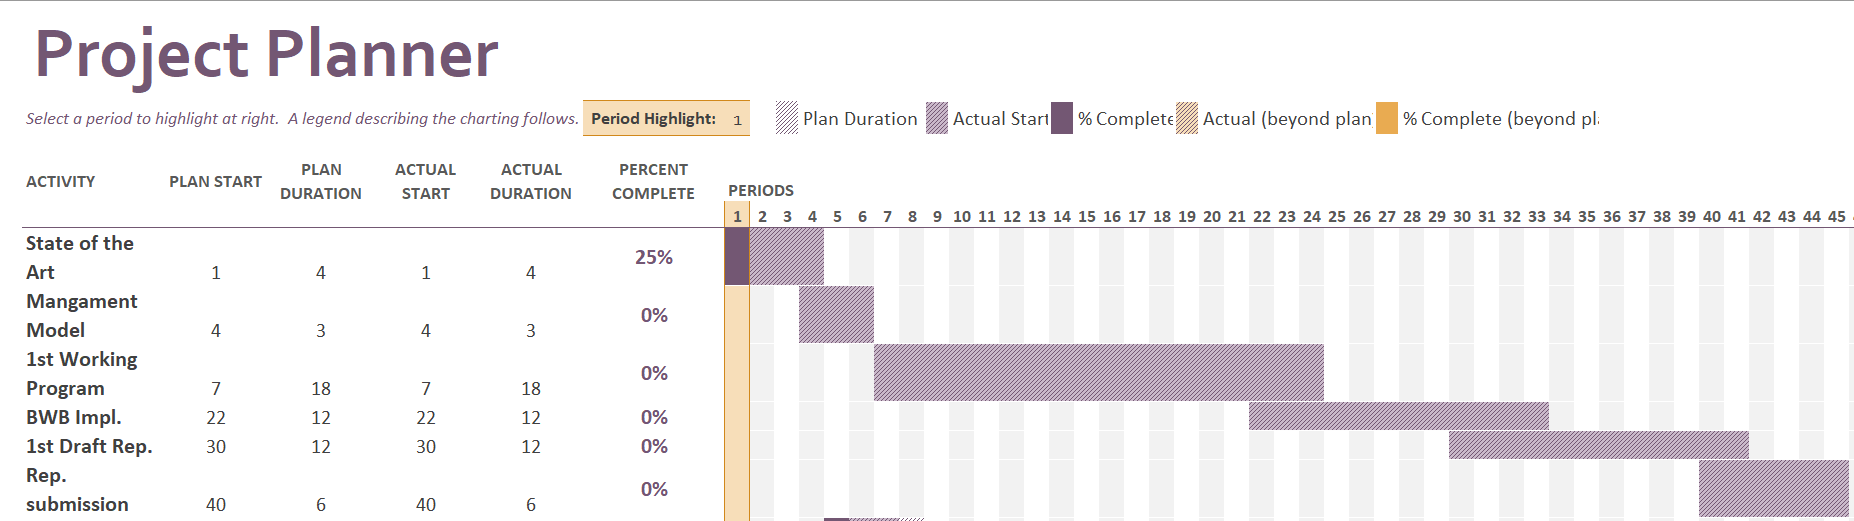
\includegraphics[width=\textwidth]{images/Gantt}
\caption{Gantt chart for the project. A period represents one week, the first week corresponds to the first week of April.}
\label{fig:gantt}
\end{sidewaysfigure}
%%% Local Variables: 
%%% mode: latex
%%% TeX-master: "isae-report-template"
%%% End: 
